\documentclass[12pt]{article}
\title{VLSI Design Algorithms}
\author{Nima Poshtiban}
\usepackage{datetime}
\newdate{date}{13}{10}{2025}
\date{\displaydate{date}}
\usepackage[utf8]{inputenc}
\usepackage{amsmath}
\usepackage{enumitem}
\usepackage{graphicx}
\usepackage[urlcolor=blue, bookmarksopen]{hyperref}
\usepackage[]{geometry}
\usepackage[]{cleveref}
\usepackage{fancyhdr}
\usepackage{xcolor}
\usepackage{siunitx}
\usepackage{tikz}
\usepackage{subcaption}
\makeindex
\hypersetup{
    colorlinks=true,
    linkcolor=blue,
    filecolor=magenta,      
    urlcolor=cyan,
    citecolor=blue,
    pdftitle={Overleaf Example},
    pdfpagemode=FullScreen,
    }
    
\urlstyle{same}

\begin{document}
\maketitle
\pagebreak
\tableofcontents
\section{VLSI Design Problems}
\paragraph{}
\textbf{Definition:}\vspace{1em}\\
{\textbf{VLSI}} is the Antonym of \textit{Very Large Scale Integration}. In general an \textbf{IC} or \textbf{technology} that contain more than \(\mathbf{10^{5}}\) transistors are considered \textbf{VLSI}. There is also \textbf{LSI} (Large Scale Integration); albeit having different spelling, they are used interchangeably. There are \textbf{six} crucial factors in VLSI Optimization.\\
\begin{enumerate}
\item Area
\item Speed
\item Power Consumption 
\item Thermal Management
\item Signal Integrity
\item Congestion
\end{enumerate}

The problem is one can not simply improve all the factors, there are trade-offs between these factors. Also \textbf{Design Time} is an important thing to consider in the economical context, it is worth mentioning that\textbf{ Testability} is an important factor to consider; because a noticeable percentage of the fabricated chips are defective, this makes testing chips a vital process before being used in the product. \\ VLSI is can be a\textbf{ general-purpose integrated circuit}(e.g. microprocessor) or an \textbf{application-specific integrated circuits(ASICs)}.
Relations between the main factor can be expressed as:\[
	\mathit{Speed}\,\alpha\,\frac{1}{\mathit{Area}}\quad \,\mathit{Power\,Consumption}\,\alpha\,\frac{1}{\mathit{Area}} 
\]
The smaller \textbf{Area} means \textbf{less silicon }consumption and increase in the\textbf{ yield}. \textit{The Larger the Area the higher chance of defects}.\\
\textbf{Speed} is a\textbf{ design constraint}, meaning optimization revolves around the designated \textbf{Speed}. 
\section{Boundary Optimization}
\paragraph{}
Definition: In simple terms \emph{Boundary Optimization} can be defined as the set of techniques
aiming for the improvement of \textbf{circuits} both in \textbf{efficiency and performance} at the boundaries between \textbf{different logic modules}
	
\paragraph{}
\textbf{Types of Boundary Optimization} \\
There are \emph{four} main types of \textbf{Boundary Optimization} 
\begin{enumerate}[label=\textcolor{blue}{\arabic*.}]
\item \textcolor{blue}{\textbf{Boundary Condition Optimization}} 
\item \textcolor{blue}{\textbf{Boundary Merging}}
\item \textcolor{blue}{\textbf{Boundary Logic Optimization}}
\item \textcolor{blue}{\textbf{Retiming}}
\end{enumerate}
\paragraph{}
\textbf{Boundary Condition Optimization} \\
This optimization is focused on improving \emph{signal integrity} while crossing from one module to another. The main benefits are:
\begin{enumerate}
\item Preventing Timing Violations
\item Better Timing Performance 
\item Power Consumption Reduction 
\end{enumerate}
\paragraph{}
\textbf{Boundary Merging} \\
This Techniques focuses on merging \textbf{adjacent blocks or modules} with \underline{similar} functionality. This techniques has several benefits:
\begin{enumerate}
\item Area Reduction
\item Reduction in Power Consumption
\item Enhance Timing
\end{enumerate}
\paragraph{}
{\textbf{Boundary Logic Optimization}} \\
As the name suggests, the technique is focused on logic redundancy elimination, thus \textbf{simplifying the logic equation complexity}. In Addition it \textbf{simplifies the design} and \textbf{Reduces the power consumption}.
\paragraph{}
\textbf{Re-timing} \linebreak
The mechanism behind \textbf{Re-timing} is based on \textit{flip-flops and registers} re-positioning; The \textbf{clock skew will be reduced} and \textbf{bottlenecks will be prevented}.
\section{Design Methodologies}
\paragraph{}
One approach for VLSI Design is using a cost function with the required factors as the inputs of the function. The General form of the cost function can be show as (\textbf{i} is a component):\[
	\mathbf{C}\,=\,\sum_{i\,=\,1}^{N}\left(\,w_{p}\\,P_{1}\,+\,w_{D}\,\frac{L_{i}}{V_{i}(t)}+w_{A}\,A_{i}\right)
\]
Where \large{\(\mathit{C}\)} is the\textbf{ cost function} and; {\large\(P_{i}\)} is the \textbf{Power Consumption} \newline
of \textbf{component i}; \large{\(\mathit{L_{i}}\)} is length of the path for the \(i\);
\large{\(V_{i}(t)\)} is the voltage of \(i\) at time \(t\); \large{\(\mathit{A_{i}}\)} is the Area of \(i\) and, \large{\(w\)} is the weight of each factor relevant to its importance (in this simplified formula \(p\) is for power, \(D\) for delay and, \(A\) for area).\newline
Designing a cost function usually tends to become more complex and time consuming as the factors grow.\\ Thereby a proper approach is necessary to reduce the complexity, this can be achieved through \textbf{Divide and Conquer} methodology by breaking down a large chip into smaller parts and abstract away the unnecessary details of the blocks \autoref{abs_main}.
\begin{figure}[b!]  
\usetikzlibrary {through}
\tikzset{auto}

\begin{tikzpicture}
	
	\node [draw] at (0,0) [circle through={(2,2)}] {$A$};
	\node [draw] at (1.2,1.2) [circle through={(2,2)}] {\(B\)};
	\node [draw] at (1.67,1.9) [circle through={(2,2)}] {\(E\)};
	\node [draw] at (0.7,1.1) [circle through={(1,1)}] {\(F\)};
	\node [draw] at (-1.2,1) [circle through={(0,1)}] {\(C\)};
\node [draw] at (-1.9,1.4) [circle through={(-1.9,1)}] {\(G\)};
\node [draw] at (-0.5,1.2) [circle through={(0,1.1)}] {\(H\)};
\end{tikzpicture}
\hspace{4em}
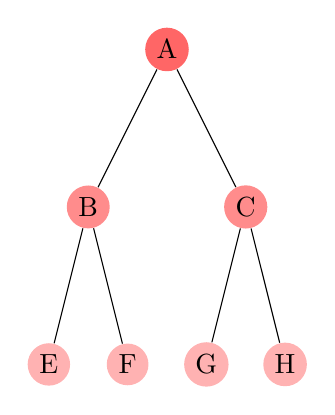
\begin{tikzpicture}
	[level distance=20mm,
	every node/.style={fill=red!60,circle,inner sep=2pt},
	level 1/.style={sibling distance=20mm,nodes={fill=red!45}},
	level 2/.style={sibling distance=10mm,nodes={fill=red!30}},
	level 3/.style={sibling distance=5mm,nodes={fill=red!25}}],
	\
	\node {A}
	child {node {B}
		child {node {E}}
		child {node {F}}
	}
	child {node {C}
		child {node {G}}			
		child {node {H}}
	};

\end{tikzpicture}
\caption{design hierarchy examples}
\label{abs_main}
\end{figure}
%TODO
%Add design domains
\bibliographystyle{ieeetr}
\bibliography{vlsi.bib}
\end{document}